\chapter{Introduzione alla sicurezza di rete}

\dfn{Sicurezza di rete}{
    La sicurezza di rete è l'insieme delle strategie, tecnologie e protocolli utilizzati per proteggere le reti di calcolatori da accessi non autorizzati, attacchi, perdite di dati e altre minacce informatiche
}

In pratica consiste nel creare un'architettura di difesa e prevenzione. Questi sono in modo riassuntivo i principali obbiettivi della sicurezza di rete:
\begin{itemize}
    \item \textbf{Confidenzialità}: Solo il mittente e il destinatario devono poter leggere il messaggio. Questo si ottiene con la crittografia
    \begin{itemize}
        \item Il mittente crittografa (encrypts) il messaggio.
        \item Il destinatario decrittografa (decrypts) il messaggio
    \end{itemize}
    \item \textbf{Autenticazione}: Processo per verificare l’identità di un utente o un dispositivo, fondamentale per garantire accessi sicuri (es. Password, certificati digitali, autenticazione a due fattori (2FA))
    \item \textbf{Integrità dei messaggi}: Garantisce che i dati non siano stati alterati durante la trasmissione (es. Password, certificati digitali, autenticazione a due fattori (2FA))
    \item \textbf{Accesso e Disponibilità}: I servizi devono essere accessibili agli utenti autorizzati. Minacce:
    \begin{itemize}
        \item Attacchi DoS/DDoS che bloccano il servizio.
        \item Gestione dei permessi per prevenire accessi non autorizzati
    \end{itemize}
\end{itemize}

Si introduce il concetto di attacco con il tipico esempio di Alice e Bob che vogliono comunicare e Trudy, l'attaccante, che può intercettare, elliminare o aggiungere messaggi durante la comunicazione dei due amamnti carucci (Morbidelli - Morigi)
\begin{center}
    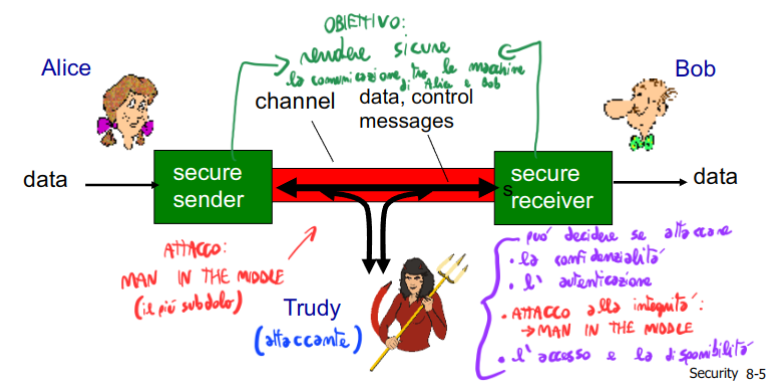
\includegraphics[width=10cm]{img/trudy_bob_alice.png}
\end{center}

Vabbuò passiamo alla sezione sucessiva:
\section{Principi di crittografa}
Partiamo dalla defnizione

\dfn{crittografa}{
    si \textbf{crittografa} la disciplina che studia le tecniche per proteggere le informazioni trasformandole in un formato illeggibile per chi non è autorizzato, consentendo solo ai destinatari legittimi di decifrarle.
}

Nelle reti di comunicazione, i dati trasmessi possono essere intercettati da chiunque abbia accesso al canale di comunicazione, rendendo le informazioni vulnerabili a lettura, modifica o attacchi malevoli. Per proteggere la riservatezza e l’integrità dei dati, si utilizza, quindi, la crittografia, una tecnica che consente di trasformare il testo in chiaro, detto \textit{plaintext}, in un formato incomprensibile chiamato testo cifrato o \textit{ciphertext}, attraverso l’applicazione di un algoritmo di cifratura.

L’obiettivo della crittografia è garantire che, anche se un malintenzionato intercettasse il messaggio durante la trasmissione, non sarebbe in grado di comprenderne il contenuto senza la conoscenza della chiave segreta. Solo il destinatario legittimo, in possesso della chiave corretta, può applicare un algoritmo di decifratura per convertire il testo cifrato nuovamente in testo leggibile.

Va sottolineato che gli algoritmi di cifratura e decifratura sono generalmente pubblici e noti a tutti. Tuttavia, la sicurezza della crittografia si basa sulla segretezza della cosiddetta \textit{chiave crittografica}, ovvero una sequenza di bit utilizzata all'interno di un algoritmo di cifratura per trasformare un messaggio in un formato sicuro e, successivamente, per riconvertirlo nel suo stato originale. Questa chiave viene generata all'inizio della comunicazione tra mittente e destinatario e loro e solo loro ne sono a conoscenza.

Adesso un'introduzione all'algebra della crittografia

Si ha:
\begin{itemize}
    \item $m$: plaintext
    \item $K_A(m)$: ciphertext, encrypted with key $K_A$
    \item $m = K_B(K_A(m))$: plaintext ripristinato grazie alla chiave $K_B$
\end{itemize}

Si noti la seguente immagine (con appunti bonziani):
\begin{center}
    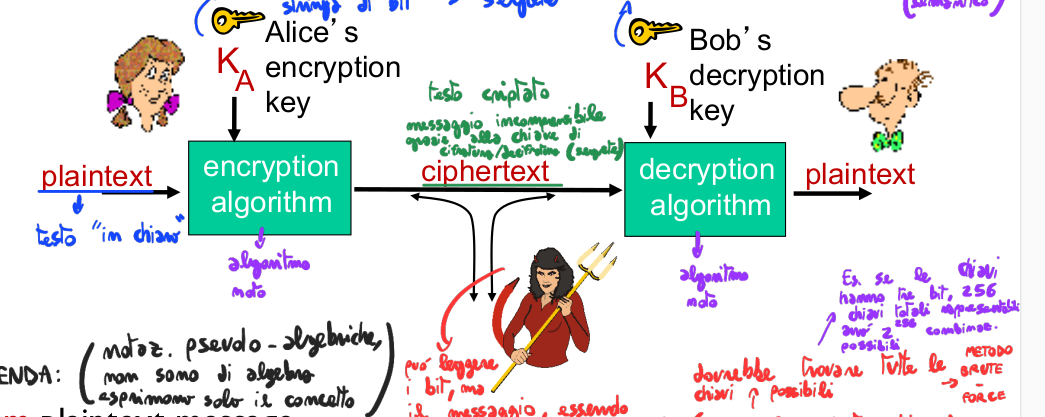
\includegraphics[width=10cm]{img/crittografia.png}
\end{center}

\subsection{Attaccare uno schema di crittografia}

Gli attacchi crittografici mirano a violare la sicurezza di un sistema di cifratura. Ne esistono diversi tipi:
\begin{enumerate}
    \item \textbf{Cipher-text only attack}, l'attaccante possiede solo il testo cifrato a disposizione e per decifrare il messaggio ha due approcci possibile:
    \begin{itemize}
        \item \textbf{Forza bruta}: prova tutte le chiavi possibili
        \item \textbf{Analisi statistica}: cerca pattern ripetuti nei dati cifrati
    \end{itemize}
    \item \textbf{known-plaintext attack}: Trudy possiede sia il testo cifrato che il corrispondente testo in chiaro. Con queste informazioni, cerca di scoprire la chiave di cifratura o il meccanismo utilizzato, così da poter decifrare altri messaggi cifrati dallo stesso sistema.
    
    \ex{}{
    Se Trudy sa che nel testo in chiaro compare la parola "hello" e trova nel messaggio cifrato la sequenza "JGRRG", può iniziare a costruire un dizionario di corrispondenze tra lettere:

    \begin{itemize}
        \item $h \to J$
        \item $e \to G$
        \item $l \to R$
        \item $o \to G$
    \end{itemize}
    }
    
\end{enumerate}

\nt{un buon metodo per evitare questi attacchi è rendere lo spazio delle chiavi il più vasto possibile e utilizzare algoritmi sicuri che resistano alle analisi statistiche}
\subsection{Crittografia a chiave simmetrica}
Adesso entriamo nel vivo della difesa cazzo
\dfn{Crittografia a chiave simmetrica}{
    mittente e destinatario condividono la stessa chiave segreta $K_S$ per cifrare e decifrare i messaggi
}

I pratica il mittente (Alice) cirfra il plaintext con l'algoritmo di cifratura usando la chiave $K_S$ottenendo il ciphertext, Bob riceve il ciphertext e lo decifra usando lo stesso algoritmo e la chiave $K_S$, recuperando il messaggio originale
\begin{center}
    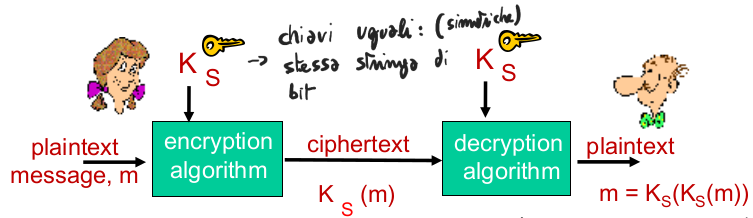
\includegraphics[width=10cm]{img/CHIAVE_SIMMETRICA.png}
\end{center}

Per implementare la chiave simmetrica esistono diverse tecniche

\subsubsection{Cifrario a sostituzione}

\dfn{Cirfrario a sostituizione}{
    Un \textbf{cifrario a sostituzione} è una tecnica di cifratura in cui ogni lettera del testo in chiaro viene sostituita con un'altra lettera secondo un mapping predefinito
}

\paragraph{Cifrario monolitico}
Tra i vari tipi di cifrario a sostruzioni vi è il cifrario monolitico dove ogni lettera dell'alfabeto viene sostituita da un'altra lettera fissa

\ex{Cifrario monolitico}{
    \begin{itemize}
        \item Alfabeto in chiaro: abcdefghijklmnopqrstuvwxyz

        \item Alfabeto cifrato: mnbvcxzasdfghjklpoiuytrewq
        \item Messaggio originale: bob. i love you. alice
        \item Messaggio cifrato: nkn. s gktc wky. mgsbc
    \end{itemize}
}

La chiave di cifratura è una funzione di permutazione ad un insieme di 26 lettere ad un altro insieme di 26 lettere

Tuttavia è poco sicuro perché mantiene la frequenza delle lettere originali e lo rende particolarmente vulnerabile alle analisi delle frequenze

\paragraph{Schema ciclico} Per rendere la cifratura più sicura, si può usare più cifrari di sostituzione e applicarli in un ciclo predefinito

La chiave di cifratura quindi è un insieme di $n$ cifrari sostituzione ($M_1,M_2,\dots,M_n$) ed un modello cicilico su come usarli. Ogni lettera del plaintext quindi viene cifrata con un cifrario diverso seguendo il ciclo 

\subsubsection{DES (Data Encryption Standard)}
Il DES è stato uno standard di crittografia a chiave simmetrica ampiamente adottato. Funziona come un \textbf{cifrario a blocchi}: il messaggio in chiaro viene suddiviso in blocchi di 64 bit, e ogni blocco viene cifrato indipendentemente utilizzando una chiave a 56 bit.

La struttura del DES prevede 16 "round" identici di elaborazione, dove ogni round utilizza una porzione diversa (48 bit) della chiave principale. Questo processo complesso di permutazioni e sostituzioni mira a offuscare la relazione tra il testo in chiaro e quello cifrato.

\nt{Oggi il DES è considerato \textbf{insicuro}. Una chiave a 56 bit è troppo corta per resistere a un attacco a forza bruta con la potenza di calcolo moderna. Nel 1998, una chiave DES fu violata in meno di un giorno.}

Per aumentarne la sicurezza, è stato introdotto il \textbf{3DES (Triple DES)}, che applica l'algoritmo DES tre volte consecutive con tre chiavi diverse, portando la dimensione effettiva della chiave a 168 bit e rendendo gli attacchi a forza bruta computazionalmente impraticabili.

\subsubsection{AES (Advanced Encryption Standard)}
L'AES è lo standard attuale che ha sostituito il DES. Come il DES, è un cifrario a blocchi, ma è più robusto e flessibile:
\begin{itemize}
    \item Elabora dati in blocchi da \textbf{128 bit}.
    \item Supporta chiavi di tre dimensioni diverse: \textbf{128, 192 o 256 bit}.
\end{itemize}
Grazie alla maggiore lunghezza della chiave, l'AES è esponenzialmente più sicuro del DES. Si stima che un attacco a forza bruta che violasse una chiave DES in 1 secondo impiegherebbe circa 149 trilioni di anni per violare una chiave AES a 128 bit.

\subsection{Crittografia a chiave pubblica (o asimmetrica)}

La crittografia a chiave pubblica rappresenta un cambio di paradigma rispetto a quella simmetrica. Il suo vantaggio principale è che \textbf{mittente e destinatario non devono condividere una chiave segreta}. Ogni utente possiede una coppia di chiavi:
\begin{itemize}
    \item Una \textbf{chiave pubblica ($K^+$)}, nota a tutti, che serve per cifrare i messaggi.
    \item Una \textbf{chiave privata ($K^-$)}, conosciuta solo dal proprietario, che serve per decifrare i messaggi.
\end{itemize}
Se Alice vuole inviare un messaggio a Bob, cifra il messaggio con la chiave pubblica di Bob ($K_B^+$). Solo Bob, in possesso della sua chiave privata ($K_B^-$), potrà decifrarlo.
\begin{center}
    \includegraphics[width=10cm]{CHIAVE_PUBBLICA.png}
\end{center}
Questo sistema si basa su \textbf{funzioni matematiche unidirezionali (one-way)}, facili da calcolare in una direzione ma computazionalmente impossibili da invertire senza informazioni aggiuntive. Un esempio è la fattorizzazione di numeri molto grandi.

\subsubsection{Algoritmo RSA (Rivest, Shamir, Adelson)}
L'algoritmo RSA è l'implementazione più nota della crittografia a chiave pubblica. La sua sicurezza si basa sulla difficoltà di fattorizzare un numero intero che è il prodotto di due numeri primi molto grandi.

\paragraph{Generazione delle chiavi}
\begin{enumerate}
    \item Scegliere due numeri primi molto grandi, $p$ e $q$.
    \item Calcolare $n = p \times q$ e $z = (p-1)(q-1)$.
    \item Scegliere un numero intero $e$ (con $e < n$) tale che non abbia fattori comuni con $z$.
    \item Calcolare un numero $d$ tale che $ed \pmod z = 1$.
    \item La \textbf{chiave pubblica} è la coppia $(n, e)$.
    \item La \textbf{chiave privata} è la coppia $(n, d)$.
\end{enumerate}

\paragraph{Cifratura e Decifratura}
Per poter applicare le operazioni matematiche, un messaggio $m$ viene prima convertito in un numero intero.
\begin{itemize}
    \item \textbf{Cifratura}: $c = m^e \pmod n$
    \item \textbf{Decifratura}: $m = c^d \pmod n$
\end{itemize}
La magia matematica assicura che $m = (m^e \pmod n)^d \pmod n$. La sicurezza risiede nel fatto che, pur conoscendo la chiave pubblica $(n, e)$, è computazionalmente infattibile determinare la chiave privata $d$ senza conoscere i fattori primi $p$ e $q$ di $n$.

\nt{Una proprietà fondamentale di RSA è che le operazioni possono essere invertite: $K_B^+(K_B^-(m)) = m$. Cifrare con la chiave privata e decifrare con quella pubblica è alla base delle \textbf{firme digitali}, usate per garantire l'autenticità.}

\subsection{L'approccio ibrido: le chiavi di sessione}

La crittografia a chiave pubblica (come RSA) è molto potente ma anche molto \textbf{lenta} e computazionalmente costosa. Al contrario, la crittografia a chiave simmetrica (come AES) è estremamente veloce.

Nella pratica, si usa quasi sempre un approccio ibrido che combina il meglio di entrambi i mondi:
\begin{enumerate}
    \item \textbf{Fase 1: Scambio della chiave.} Alice e Bob usano la crittografia a chiave pubblica (lenta ma sicura) per scambiarsi una chiave simmetrica temporanea, detta \textbf{chiave di sessione ($K_S$)}.
    \item \textbf{Fase 2: Comunicazione.} Una volta che entrambi possiedono $K_S$, usano la crittografia simmetrica (veloce ed efficiente) con quella chiave per tutta la durata della loro comunicazione.
\end{enumerate}

Questo approccio risolve il problema della condivisione della chiave della crittografia simmetrica, mantenendo al contempo alte prestazioni per lo scambio di grandi quantità di dati.
\section{Integrità del Messaggio e Autenticazione}
Oltre alla confidenzialità, è cruciale garantire che il messaggio non sia stato alterato e che l'identità degli interlocutori sia certa.

\subsection{Autenticazione}
L'obiettivo è permettere a Bob di essere sicuro che sta comunicando con la vera Alice. Protocolli semplici sono insicuri:
\begin{itemize}
    \item "Sono Alice": Trudy può semplicemente mentire.
    \item "Sono Alice" con IP di Alice: Trudy può falsificare (spoof) l'indirizzo IP del mittente.
    \item Invio della password in chiaro: Trudy può intercettare la password e riutilizzarla in un \textbf{playback attack}.
\end{itemize}

Per evitare i playback attack, si usa una tecnica di \textbf{challenge-response} con un \textit{nonce}.

\dfn{Nonce}{
    Un numero casuale (R) che viene utilizzato una sola volta (\textit{Number used once}) in una sessione di comunicazione.
}

Il protocollo diventa:
\begin{enumerate}
    \item Alice si annuncia a Bob.
    \item Bob le invia un nonce casuale R.
    \item Alice deve cifrare R con una chiave segreta condivisa e inviarlo a Bob. Poiché R è nuovo per ogni sessione, Trudy non può riutilizzare una risposta registrata in passato. Questo prova che Alice è "live" e conosce la chiave segreta.
\end{enumerate}

Questo approccio, seppur efficace per l'autenticazione, è vulnerabile a un attacco \textbf{Man-in-the-Middle (MitM)} se la chiave pubblica usata non è certificata.

\subsection{Firme Digitali e Funzioni Hash}
La crittografia a chiave pubblica ha un'altra proprietà fondamentale: $K_B^{+}(K_B^{-}(m)) = m$. Cifrare con la chiave privata e decifrare con quella pubblica funziona, ed è la base della \textbf{firma digitale}.

\dfn{Firma Digitale}{
    Una tecnica crittografica che permette a un mittente di "firmare" un documento digitale per garantirne l'autenticità, l'integrità e il non ripudio (il mittente non può negare di averlo firmato).
}

Poiché cifrare un intero messaggio con RSA è lento, non si firma il messaggio, ma un suo "riassunto" di dimensione fissa, chiamato \textit{message digest}.

\dfn{Funzione Hash Crittografica}{
    Un algoritmo matematico (es. MD5, SHA-1) che prende in input un messaggio di lunghezza arbitraria e produce un output di lunghezza fissa (es. 128 o 160 bit), detto \textbf{hash} o \textbf{message digest}. Deve essere computazionalmente impossibile trovare due messaggi diversi che producano lo stesso hash.
}

Il processo di firma digitale diventa:
\begin{enumerate}
    \item Bob calcola l'hash del suo messaggio, $H(m)$.
    \item Bob cifra l'hash con la sua \textbf{chiave privata}, $K_B^-(H(m))$. Questo è la firma.
    \item Bob invia ad Alice il messaggio in chiaro $m$ e la firma $K_B^-(H(m))$.
    \item Alice riceve il tutto, ricalcola autonomamente l'hash del messaggio $m$, e decifra la firma usando la \textbf{chiave pubblica di Bob}, $K_B^+(K_B^-(H(m)))$.
    \item Se i due hash coincidono, Alice ha la certezza che il messaggio proviene da Bob e non è stato alterato.
\end{enumerate}

\subsection{Autorità di Certificazione (Certification Authorities - CA)}
Resta un problema: come fa Alice ad essere sicura che la chiave pubblica che sta usando per verificare la firma di Bob appartenga davvero a Bob e non a Trudy? La soluzione sono le Autorità di Certificazione.

\dfn{Certification Authority (CA)}{
    Un'entità terza fidata (es. Verisign, Let's Encrypt) che ha il compito di associare un'identità a una chiave pubblica.
}

Una CA emette un \textbf{certificato digitale}, che è un documento elettronico contenente l'identità di un'entità (es. Bob), la sua chiave pubblica, e altri dati. L'intero certificato è \textbf{firmato digitalmente dalla CA} con la propria chiave privata.

Quando Alice vuole comunicare con Bob, lui le invia il suo certificato. Alice, che si fida della CA e possiede la chiave pubblica della CA, può verificare la firma sul certificato. Se la verifica ha successo, Alice è certa che la chiave pubblica contenuta nel certificato appartiene legittimamente a Bob, sventando così l'attacco Man-in-the-Middle.

\section{Mettere in Sicurezza l'E-mail}
Un'applicazione come la posta elettronica richiede di garantire tutti e tre i pilastri della sicurezza: confidenzialità, autenticazione e integrità. Questo si ottiene combinando in modo intelligente la crittografia simmetrica e quella asimmetrica.

\subsection{Confidenzialità per l'E-mail}
Per inviare un messaggio confidenziale $m$ a Bob, Alice non usa direttamente la lenta crittografia a chiave pubblica per cifrare l'intero messaggio. Adotta invece un approccio ibrido:
\begin{enumerate}
    \item Alice genera una \textbf{chiave di sessione simmetrica} casuale, $K_S$.
    \item Usa la veloce crittografia simmetrica per cifrare il messaggio: $K_S(m)$.
    \item Usa la lenta crittografia a chiave pubblica per cifrare solo la chiave di sessione, utilizzando la \textbf{chiave pubblica di Bob}: $K_B^+(K_S)$.
    \item Alice invia a Bob entrambi gli elementi: il messaggio cifrato e la chiave di sessione cifrata.
\end{enumerate}

Quando Bob riceve il tutto:
\begin{enumerate}
    \item Usa la sua \textbf{chiave privata} per decifrare e recuperare la chiave di sessione: $K_B^-(K_B^+(K_S)) = K_S$.
    \item Usa la chiave di sessione $K_S$ appena recuperata per decifrare il messaggio: $K_S(K_S(m)) = m$.
\end{enumerate}

\subsection{Autenticazione e Integrità per l'E-mail}
Per garantire l'autenticità e l'integrità, Alice utilizza una firma digitale:
\begin{enumerate}
    \item Calcola un \textit{message digest} del messaggio tramite una funzione hash: $H(m)$.
    \item Cifra l'hash con la sua \textbf{chiave privata} per creare la firma: $K_A^-(H(m))$.
    \item Invia a Bob il messaggio in chiaro $m$ insieme alla firma digitale.
\end{enumerate}

Bob può verificare la firma utilizzando la chiave pubblica di Alice, garantendo così che il messaggio provenga da lei e non sia stato alterato.

\subsection{Combinare tutte le Proprietà di Sicurezza}
Per ottenere contemporaneamente confidenzialità, autenticazione e integrità, Alice combina i due processi: firma prima il messaggio e poi cifra il tutto.

% \begin{center}
%     \includegraphics[width=14cm]{img/secure_email_combined.png}
% \end{center}

\section{Mettere in Sicurezza le Connessioni TCP: SSL/TLS}
Mentre la sicurezza dell'e-mail protegge il contenuto "a riposo", è spesso necessario proteggere i dati "in transito" per qualsiasi applicazione che utilizzi TCP. La soluzione standard per questo è SSL.

\dfn{SSL (Secure Sockets Layer)}{
    Un protocollo che fornisce un canale di comunicazione sicuro, inserendosi tra il livello Applicazione e il livello Trasporto (TCP). Fornisce confidenzialità, integrità e autenticazione a qualsiasi applicazione basata su TCP. La sua versione moderna e standardizzata è chiamata \textbf{TLS (Transport Layer Security)}.
}

SSL è la tecnologia alla base di \textbf{HTTPS}. È supportato da quasi tutti i browser e server web e viene utilizzato per proteggere miliardi di transazioni ogni giorno.

\subsection{Funzionamento di SSL}
SSL opera in due fasi principali:
\begin{enumerate}
    \item \textbf{Handshake Phase}: È una fase di negoziazione iniziale in cui client e server si autenticano a vicenda (tipicamente, il server si autentica al client tramite un certificato digitale), concordano gli algoritmi crittografici da utilizzare e generano le chiavi di sessione simmetriche che verranno usate per la comunicazione.
    \item \textbf{Data Transfer Phase}: I dati dell'applicazione vengono frammentati in record. Ogni record viene protetto con un MAC (Message Authentication Code) per garantirne l'integrità e poi cifrato con la chiave di sessione simmetrica per garantirne la confidenzialità, prima di essere passato a TCP per la trasmissione.
\end{enumerate}

\paragraph{Il protocollo di Handshake}
L'handshake è il cuore di SSL e stabilisce la connessione sicura. In sintesi:
\begin{enumerate}
    \item Il client invia un messaggio `ClientHello` con una lista di suite crittografiche che supporta e un numero casuale (nonce).
    \item Il server sceglie una suite dalla lista, invia un `ServerHello`, il suo certificato digitale (contenente la sua chiave pubblica) e un suo nonce.
    \item Il client verifica il certificato del server (usando la chiave pubblica della CA). Se valido, genera un segreto condiviso (\textit{pre-master secret}), lo cifra con la chiave pubblica del server e glielo invia.
    \item A questo punto, sia client che server, utilizzando i due nonce e il pre-master secret, derivano in modo indipendente lo stesso insieme di chiavi di sessione (per cifratura e MAC in entrambe le direzioni).
    \item La fase si conclude con lo scambio di messaggi `Finished`, cifrati con le nuove chiavi, che confermano che l'handshake è avvenuto correttamente e senza manomissioni.
\end{enumerate}

\section{Sicurezza a Livello Rete: IPsec}
SSL/TLS è ottimo per proteggere singole applicazioni, ma cosa succede se si vuole fornire una "copertura di sicurezza" generale a tutto il traffico che esce da un host o da un'intera rete? A questo scopo, si opera a un livello più basso, il Livello 3, con il protocollo \textbf{IPsec}.

\dfn{IPsec (IP Security)}{
    Una suite di protocolli che fornisce sicurezza a livello di pacchetti IP. Può cifrare e/o autenticare tutto il traffico IP, indipendentemente dall'applicazione (TCP, UDP, ICMP, ecc.). È la tecnologia fondamentale per la creazione di \textbf{Virtual Private Networks (VPN)}.
}

\dfn{VPN (Virtual Private Network)}{
    Una rete che utilizza l'infrastruttura di una rete pubblica (come Internet) per trasportare traffico di una rete privata, mantenendolo logicamente separato e sicuro tramite cifratura e "tunnelling". Ad esempio, permette a un'azienda di collegare in modo sicuro la sua sede centrale e una filiale, facendo viaggiare i dati su Internet come se fossero su una linea privata.
}

\subsection{Protocolli e Modalità di IPsec}
IPsec offre flessibilità attraverso due protocolli e due modalità operative:
\begin{itemize}
    \item \textbf{Protocolli IPsec}:
    \begin{itemize}
        \item \textbf{AH (Authentication Header)}: Fornisce autenticazione dell'origine e integrità dei dati, ma \textit{non} la confidenzialità (i dati non sono cifrati).
        \item \textbf{ESP (Encapsulating Security Payload)}: Fornisce autenticazione, integrità \textit{e} confidenzialità. È il protocollo più utilizzato.
    \end{itemize}
    \item \textbf{Modalità Operative}:
    \begin{itemize}
        \item \textbf{Transport Mode}: Cifra solo il payload del pacchetto IP (es. il segmento TCP), lasciando l'header IP originale in chiaro. Viene usato per proteggere la comunicazione tra due host finali.
        \item \textbf{Tunnel Mode}: Cifra l'intero pacchetto IP originale (header incluso), e lo "incapsula" in un nuovo pacchetto IP con un nuovo header. È la modalità utilizzata per le VPN tra router.
    \end{itemize}
\end{itemize}

% \begin{center}
%     \includegraphics[width=13cm]{img/IPsec_VPN_diagram.png}
% \end{center}

\subsection{Security Associations (SA)}
A differenza di IP, che è connectionless, IPsec è \textbf{connection-oriented}. Prima che due entità possano scambiarsi dati protetti, devono stabilire una \textbf{Security Association (SA)}.

\dfn{Security Association (SA)}{
    Un accordo unidirezionale tra due entità che definisce tutti i parametri di sicurezza per il loro traffico, come il protocollo da usare (ESP o AH), gli algoritmi di cifratura e autenticazione, le chiavi e la loro durata. Per una comunicazione bidirezionale sono necessarie due SA (una per ogni direzione).
}

La configurazione manuale delle SA è impraticabile in reti complesse. Per questo, si utilizza il protocollo \textbf{IKE (Internet Key Exchange)} per negoziare e stabilire le SA in modo automatico e sicuro.
\section{Mettere in Sicurezza le LAN Wireless (IEEE 802.11)}
Le reti wireless presentano sfide di sicurezza uniche, poiché il loro mezzo trasmissivo (le onde radio) è intrinsecamente aperto e accessibile a chiunque si trovi nel raggio di copertura, rendendo l'intercettazione molto più semplice rispetto a una rete cablata.

\subsection{WEP (Wired Equivalent Privacy) e le sue vulnerabilità}
Il primo standard di sicurezza per le reti Wi-Fi fu il WEP. Il suo obiettivo era fornire un livello di privacy paragonabile a quello di una rete cablata, ma il suo design si rivelò catastroficamente fallimentare.

WEP utilizza la crittografia a flusso (RC4) con una chiave simmetrica condivisa. Per evitare di usare sempre lo stesso flusso di cifratura, combina la chiave segreta con un \textbf{Initialization Vector (IV)} di 24 bit, che dovrebbe essere unico per ogni pacchetto. L'IV viene trasmesso in chiaro insieme al pacchetto cifrato.

Le sue debolezze fatali sono:
\begin{itemize}
    \item \textbf{Spazio dell'IV troppo piccolo}: Un IV a 24 bit è estremamente corto. Su una rete trafficata, la riutilizzazione dello stesso IV è garantita in poche ore o addirittura minuti.
    \item \textbf{IV trasmesso in chiaro}: Un attaccante può facilmente rilevare quando un IV viene riutilizzato.
    \item \textbf{Vulnerabilità della crittografia a flusso}: Se un attaccante conosce il testo in chiaro di un pacchetto cifrato con un certo IV, può calcolare il keystream corrispondente a quell'IV. Quando lo stesso IV viene riutilizzato, l'attaccante può usare il keystream che ha scoperto per decifrare il nuovo pacchetto.
\end{itemize}

Queste falle hanno reso il WEP completamente insicuro e obsoleto.

\subsection{802.11i (WPA2/WPA3): la Sicurezza Moderna}
Per rimediare alle falle del WEP, è stato introdotto lo standard \textbf{IEEE 802.11i}, commercialmente noto come \textbf{WPA2} (e il suo successore \textbf{WPA3}). Questo standard fornisce un meccanismo di sicurezza robusto, che include:
\begin{itemize}
    \item Algoritmi di crittografia forti (come AES).
    \item Meccanismi robusti per l'autenticazione degli utenti e la distribuzione delle chiavi.
\end{itemize}

In un ambiente aziendale, l'autenticazione non è gestita direttamente dall'Access Point (AP), ma viene delegata a un \textbf{Authentication Server (AS)} separato. Il processo avviene in più fasi, durante le quali il client (STA) e il server di autenticazione si autenticano a vicenda e derivano in modo sicuro una gerarchia di chiavi temporanee utilizzate per cifrare i dati della sessione.

\section{Sicurezza Operativa: Firewall e IDS}
Oltre alla crittografia, la sicurezza di una rete si basa su strumenti operativi che ne controllano i confini e ne monitorano il traffico.

\subsection{Firewall}

\dfn{Firewall}{
    Un sistema di sicurezza hardware o software che agisce come un filtro al perimetro di una rete, isolando la rete interna "fidata" dalla rete esterna "non fidata" (Internet). Ispeziona il traffico in entrata e in uscita e decide se bloccarlo o lasciarlo passare in base a un insieme di regole di sicurezza predefinite.
}

% \begin{center}
%     \includegraphics[width=10cm]{img/firewall_diagram.png}
% \end{center}

I firewall sono essenziali per:
\begin{itemize}
    \item Prevenire attacchi come il \textbf{Denial of Service (DoS)}.
    \item Impedire accessi non autorizzati ai dati interni.
    \item Applicare policy di accesso, consentendo la comunicazione solo agli utenti e ai servizi autorizzati.
\end{itemize}

Esistono tre tipi principali di firewall:
\begin{enumerate}
    \item \textbf{Stateless Packet Filter}: È il tipo più semplice. Esamina ogni pacchetto individualmente, senza tenere traccia delle connessioni. La decisione di inoltrare o bloccare si basa su regole definite in una \textbf{Access Control List (ACL)}, che filtrano in base a indirizzi IP, numeri di porta e flag TCP.
    \item \textbf{Stateful Packet Filter}: È un firewall più intelligente. Tiene traccia dello stato di ogni connessione TCP attiva. Ad esempio, permette l'ingresso di un pacchetto con il flag ACK impostato solo se questo appartiene a una connessione legittimamente avviata dall'interno. Questo lo rende molto più efficace contro tecniche di scansione e attacchi di spoofing.
    \item \textbf{Application Gateway (Proxy Firewall)}: È il tipo più sofisticato, in quanto opera a livello applicazione. Invece di far comunicare direttamente client e server, agisce da intermediario. Poiché comprende il protocollo applicativo (es. HTTP), può ispezionare il contenuto dei dati e applicare regole molto più granulari, ad esempio bloccando l'upload di certi tipi di file o filtrando comandi specifici.
\end{enumerate}

\subsection{Intrusion Detection Systems (IDS)}
Mentre un firewall applica regole per prevenire attacchi, un IDS si concentra sul rilevarli mentre accadono.

\dfn{Intrusion Detection System (IDS)}{
    Un dispositivo o software che monitora il traffico di rete o i sistemi alla ricerca di attività malevole o violazioni delle policy. A differenza di un firewall, il suo scopo principale non è bloccare, ma \textbf{rilevare e allertare}.
}

Le tecniche utilizzate dagli IDS includono:
\begin{itemize}
    \item \textbf{Deep Packet Inspection}: Analisi del contenuto (payload) dei pacchetti alla ricerca di "firme" corrispondenti a virus o attacchi noti.
    \item \textbf{Analisi Correlata}: Esame del traffico su più pacchetti per identificare pattern sospetti che un firewall tradizionale non vedrebbe, come una scansione delle porte, un tentativo di mappatura della rete o un attacco DoS distribuito.
\end{itemize}

Gli IDS sono spesso dispiegati in congiunzione con i firewall per fornire una difesa a più livelli, offrendo visibilità sulle minacce che potrebbero superare i filtri perimetrali.



\section{Firewall e IDS}

Innanzi definiamo che cos'è un \textit{Firewall}

\dfn{Firewall}{
        Si definisce \textbf{Firewall} un sistema di sicurezza che isola una rete interna di un'organizzazione da internet, controllando e filtrando il traffico di rete in entrata e uscita in base a regole di sicurezza definite dette di \texttt{ACCESS} o \texttt{DENIED}
}

L'idea del Firewall è che l'esterno di una rete è composta dai cosiddetti "cattivi ragazzi" che la mamma non vi raccomanderebbe come compagni d'uscita, mentre l'interno della rete è composta da "bravi ragazzi" di cui fidarsi, lo scopo del sistema è, quindi, separare i buoni dai cattivi

\begin{center}
    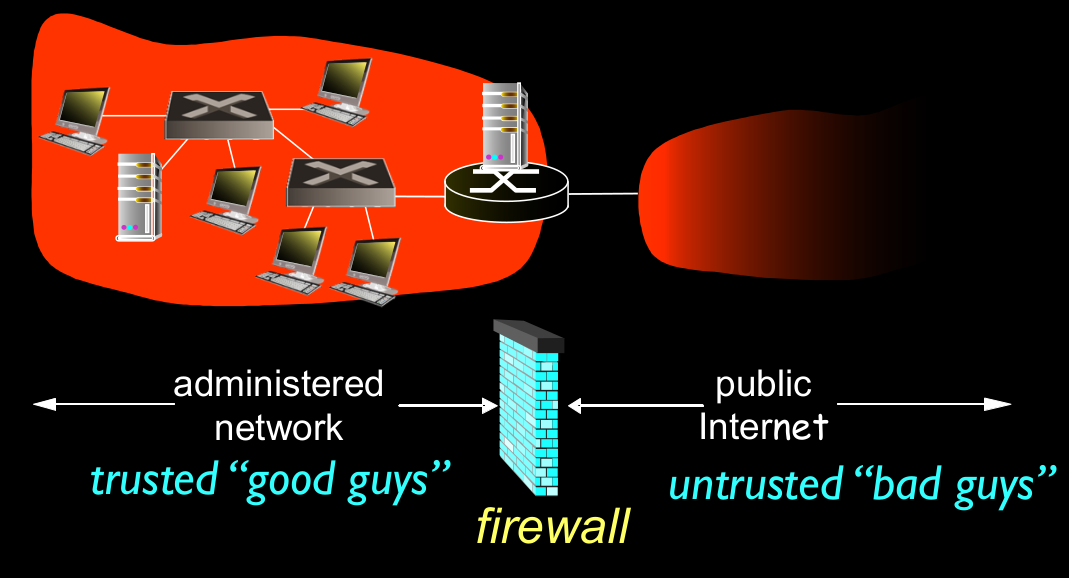
\includegraphics[width=10cm]{img/buoni_cattivi_e_firewall.png}
\end{center}

Il Firewall si rivela utile per principalmente tre motivi:
\begin{itemize}
    \item \textbf{Prevenzione degli attacchi Denial of Service (Dos)}: tipologia di attacco informatico che mira a rendere inaccessibili o indisponibili i servizi di una rete ad utenti legittimi
    
    Un esempio è il \textbf{SYN flooding} in cui un attaccante invia molte richieste di connessione false, esaurendo le risorse del server sovraccaricandolo e impedendo connessioni legittime

    \item \textbf{Protezione dei dati interni da accessi non autorizzati}: ovvero impedisce che gli attaccanti possona \textit{modificare o rubare dati sensibili}
    
    Un esempio classico è un attaccante che sostituisce il sito web di un'organizzazione con un contenuto malevolo.

    \item \textbf{Accesso selettivo e autorizzato alla rete interna}: Permette l’accesso solo a utenti o dispositivi autenticati, migliorando la sicurezza
\end{itemize}

Esistono tre tipi di tipoligie di Firewall che approfonoidremo nel dettaglio:
\begin{itemize}
    \item \textbf{Stateless Packet Filter}: Controlla ogni pacchetto singolarmente, senza tenere traccia delle connessioni
    \item \textbf{Statefull Packet Filter}: Tiene traccia dello stato delle connessioni (es. richieste e risposte)  
    \item \textbf{Application Gateway} (proxy Firewall): controlla il traffico a livello applicativo (es. HTTP, FTP, e.mail), filtrando così le informazioni che all'interno dei protocolli del livello (ad esempio il contenuto di una mail)
\end{itemize}

Si notino nel dettaglio
\subsection{Stateless Packet Filtering}

\dfn{Stateless Packet Filtering}{
    Lo \textbf{Stateless Packet Filtering} è una tecnica di sicurezza di rete in cui un firewall esamina ogni pacchetto individualmente, senza tener conto delle connessioni stabilite in precedenza. Questo significa che ogni pacchetto è valutato isolatamente sulla base di un insieme di regole predefinite
}
Di solito un firewall con filtraggio stateless è implementato su un router che collega una rete interna a internet. Il router analizza ogni pacchetto in ingresso e in uscita e decide se bloccarlo o lasciarlo in base a regole definite nelle cosiddette "\textbf{white list}" (pacchetti che possono passare) e o "\textbf{black list}" (lista di pacchetti da bloccare)

Il firewall prende decisioni basandosi su parametri del pacchetto, tra cui:
\begin{itemize}
    \item \textbf{IP} del mittente e destinatario
    \item \textbf{Numero di porta TCP/UDP} del mittente e destinatario
    \item \textbf{Tipo di messaggio ICMP} bloccando, ad esempio, attacchi di scansione provenienti dall'esterno
    \item \textbf{bit SYN e ACK nei pacchetti TCP}: Il firewall può, ad esempio, bloccare pacchetti con SYN in entrata per impedire connessioni indesiderate dall'esterno
\end{itemize}

Qui degli esempietti:
\ex{Bloccare tutti i pacchetti con protocollo UDP o Telnet}{
    \begin{itemize}
        \item \textbf{Regola}: blocca i pacchetti in entrata e in uscita se il protocollo IP è 17 (UDP) e se con la porta di origine o desitinazione è 23
        \item \textbf{Risultato}: Tutto il traffico UDP  e telnet vengono bloccati
    \end{itemize}
}

\ex{Bloccare pacchetti TCP in ingresso con ACK=0}{
    \begin{itemize}
        \item \textbf{Regola}: blocca tutti i pacchetti TCP in ingresso se il bit ACK = 0
        \item \textbf{Risultato}:Le connessioni in entrata non possono essere iniziate da un host esterno verso la rete interna e le connessioni in uscita funzionano normalmente, perché il traffico di ritorno (che ha ACK=1) è consentito.
    \end{itemize}
}

Riporto qui una tabella con altri esempi:
\begin{center}
    \begin{tabularx}{\textwidth}{|X|X|}
        \hline
        \textbf{Politica} & \textbf{Impostazione Firewall} \\
        \hline
        Nessun accesso Web esterno. & Elimina tutti i pacchetti in uscita verso qualsiasi indirizzo IP, porta 80 \\
        \hline
        Nessuna connessione TCP in entrata, tranne quelle per il server Web pubblico dell'istituzione. & Elimina tutti i pacchetti TCP SYN in entrata verso qualsiasi IP tranne 130.207.244.203, porta 80 \\
        \hline
        Impedisci alle Web-radio di consumare la larghezza di banda disponibile. & Elimina tutti i pacchetti UDP in entrata - tranne DNS e broadcast del router. \\
        \hline
        Impedisci alla tua rete di essere utilizzata per un attacco DoS smurf. & Elimina tutti i pacchetti ICMP diretti a un indirizzo di “broadcast” (ad esempio, 130.207.255.255). \\
        \hline
        Impedisci alla tua rete di essere tracciata & Elimina tutto il traffico ICMP TTL scaduto in uscita \\
        \hline
        \end{tabularx}
\end{center}

\subsubsection{Access control list}
\dfn{Liste di controllo d'accesso}{
    Le \textbf{ACL} sono tabelle di regole applicate, \textit{con priorità dall'alto verso il basso}, ai pacchetti in arrivo per decidere se consentire (allow) o bloccare (deny) il traffico di rete
}

Queste tabelle sono il vero e proprio cuore pulsante del Firewall e indicano quale pacchetto può passare e chi no
\ex{ACL}{
    \begin{center}
        \begin{tabularx}{0.5\textwidth}{|l|l|l|l|l|l|l|}
            \hline
            \textbf{azione} & \textbf{indirizzo sorgente} & \textbf{indirizzo destinazione} & \textbf{protocollo} & \textbf{porta sorgente} & \textbf{porta destinazione} & \textbf{flag bit} \\
            \hline
            allow & 222.22/16 & outside of 222.22/16 & TCP & $>$ 1023 & 80 & any \\
            \hline
            allow & outside of 222.22/16 & 222.22/16 & TCP & 80 & $>$ 1023 & ACK \\
            \hline
            allow & 222.22/16 & outside of 222.22/16 & UDP & $>$ 1023 & 53 & --- \\
            \hline
            allow & outside of 222.22/16 & 222.22/16 & UDP & 53 & $>$ 1023 & --- \\
            \hline
            deny & all & all & all & all & all & all \\
            \hline
        \end{tabularx}
            
    \end{center}
}
\subsubsection{Criticità}
Un serio problema dei Firewall Stateless che potrebbero lasciare passare pacchetti che non hanno senso nel contesto di una connessione.
Esempio:
\begin{itemize}
    \item Un pacchetto con destinazione porta 80 (HTTP) e ACK=1 arriva dall'esterno
    \item Il firewall stateless lo accetta, anche se nessuna connessione HTTP è stata avviata da un client interno.
    \item Un attaccante potrebbe sfruttare questa debolezza per inviare pacchetti falsi alla rete interna
\end{itemize}

Per porre rimedio a questi tipi di problemi si veda la tipoligia di firewall sucessiva

\subsection{Stateful packet filtering}
\dfn{Stateful packet filtering}{
    Lo \textbf{Stateful packet filtering} è una tecnica di filtraggio di pacchetti tenendo traccia delle connessioni attive e delle loro fasi
}
Un firewall stateful tiene traccia di ogni connessione TCP attiva e controlla le tre fasi fondamentali della connessione TCP (assicurandosi che ogni pacchetto in entrata o uscita abbia senso):
\begin{itemize}
    \item \textbf{Setup}: Il firewall rileva il pacchetto SYN iniziale, segnalando l'inizio di una connessione
    \item \textbf{Trasferimento dati}: I pacchetti con ACK vengono accettati solo se appartengono a una connessione già avviata
    \item \textbf{Chiusura}: Quando un pacchetto FIN o un timeout segna la fine di una connessione, il firewall non accetta più pacchetti fino a che non se apre un altro
\end{itemize}


